\documentclass{article}
\usepackage[spanish]{babel}
\usepackage{array}
\usepackage{tabularx}
\usepackage[utf8]{inputenc}
\usepackage{graphicx}
\graphicspath{ {./images/} }
\usepackage{hyperref}
\usepackage{subcaption}
\usepackage{geometry} % see geometry.pdf on how to lay out the page. There's lots.
\geometry{a4paper} % or letter or a5paper or ... etc
% \geometry{landscape} % rotated page geometry

% See the ``Article customise'' template for come common customisations

 
\author{Tomás Bacigalupo , Lucio Pagni}
\date{\today}
\author{Tomás Bacigalupo y Lucio Pagni}
\date{18/07/2020} % delete this line to display the current date

%%% BEGIN DOCUMENT
\begin{document}

% caratula
\begin{titlepage}
\centering
{
\includegraphics[width=1\textwidth]{./images/logoitba.png}\par}
\vspace{1cm}
{\scshape\Large Simulación de Sistemas \par}
\vspace{3cm}
{\scshape\Huge El problema de la distancia social en los supermercados \par}
\vspace{3cm}
{\itshape\Large Trabajo Práctico Final \par}
\vfill
{\Large Autores: \par}
{\Large Grupo 8\par}
{\Large Tomás Bacigalupo, Lucio Pagni\par}
\vfill
{\Large \today \par}
\end{titlepage}
\clearpage

\listoffigures   % generate list of figures
\clearpage
\listoftables % generate list of tables    
 \clearpage

\tableofcontents
\clearpage

\section{Introducción}

\paragraph{}
Con el objetivo de estudiar el problema de distanciamiento social en el contexto de la pandemia mundial del covid-19 se trabajó durante la segunda mitad del cuatrimestre en un software de simulación de peatones comprando en un supermercado. Dicho software busca ser más poderoso y configurable que otras versiones comerciales, las cuales usamos como referencia.

\paragraph{}
Nuestro trabajo en el desarrollo fue el de estructurar el proyecto, implementar el main (del cual se desencadenan las llamadas a todos los demás módulos),  y desarrollar el modulo de la caja, cuya tarea es la  de atender clientes y encolarlos en la fila correcta.

\paragraph{}
Por otro lado el trabajo de estructura nos llevo a tomar decisiones como desarrollos de pom.xml con sus respectivas dependencias en cada modulo y como tarea principal se implementaron todos los módulos a través de un main que permitía mediante un archivo de configuración establecer las variables de la simulación. Y es en este momento donde comienza nuestro trabajo de desarrollo para esta entrega final, donde se mejoraron los tiempos de simulación mediante la optimización de nuestros dos módulos: Main y Caja.

\section{Fundamentos}

\subsection{Main}

\paragraph{}
La idea básica del main consiste en recorrer la lista de agentes y actualizarlos. Una vez que se actualizan todos, se actualiza la lista de agentes anterior por la nueva lista de agentes. Por último el main también debe levantar un archivo de configuración.

\subsubsection{Input}

\paragraph{}

Los inputs del main provienen de la lectura de un archivo de configuración en la cual se especifican todos los valores que son parametrizables en el main. En cuanto al main, los más relevantes son el tiempo total a simular, el numero de agentes, el dt  y el dt2.

\subsubsection{Output}

\paragraph{}
El main debe guardar el estado del sistema, esto se hace cada cierto dt2, el cual es independiente del dt de simulación. Estos son archivos en los cuales se persisten información relevante de los agentes según el dt2. La información persistida en memoria mediante archivos contiene información como el id del agente, sus variables de estado (posición , velocidad) y el estado en el cual se encuentra. Esto permite un posterior procesamiento de los datos. Si bien representamos los estados con un String internamente en el simulador, en el output para procesamiento no es deseable tener un string ya que el tamaño de la salida sería muy grande innecesariamente. Es por esto que también las variables de estado se imprimieron con dos decimales. El mapeo de los estados String a número puede verse en la tabla \ref {Representación numérica de los estados en los archivos de salida}.


\subsection{Módulo Fila}

\paragraph{}
El módulo de fila se descompone en N cajas las cuales tienen 2 cajeros cada una. Tiene una capacidad máxima max, una distancia social d y una distancia H a un punto pi el cual parametriza la posición de las cajas.

\paragraph{}
La parametrización geométrica se hizo lo mas general posible para poder adaptarnos a la hora de llamar al módulo de geometría y poder usar el retorno para asignar los parámetros de nuestra implementación. En la imágen \ref{supermercado} podemos ver un plano que muestra estos parámetros. El módulo geometría expone su API en la interfaz \ref{interfaceGeomety}

\paragraph{}
El módulo provee una API pensada para la máquina de estados. Esto puede verse en \ref{interfaceCaja}

\subsubsection{Input}

\paragraph{}
El módulo fila obtiene sus inputs del módulo geometría. Obtiene de este módulo las posiciones de los lugares de pago. A partir de estos valores calcula todas las posiciones asignadas durante la simulación.

\subsubsection{Output}

\paragraph{}
El output del módulo fila se obtiene mediante su API , esto es, mediante su interfaz. Llamando a estos métodos se obtienen los estados internos de caja. El rol del módulo caja es representar mediante estructuras y algoritmos internos los estados y manejar según la lógica planteada, los agentes que manipula.


\section{Implementación}

\paragraph{}
En esta sección discutiremos todos los aspectos que hacen a la implementación del simulador y la justificación de las decisiones tomadas, tanto de diseño de clases como de diseño de arquitectura.

\subsection{Estructura, herramientas y frameworks}

\paragraph{}
El lenguaje de programación utilizado es Java , versión 8. Se utilizó JUnit como framework de testing, para tener cierto nivel de confianza y seguridad en el código implementado. Para estructurar los archivos del proyecto se utilizo la herramienta maven. Para visualizar durante la etapa de desarrollo se utilizo Ovito y también un animador en Python.

\subsection{La estructura general del proyecto}

\paragraph{}
En cuanto a la estructura, se optó por una implementación simple de Interfaces e Implementaciones, con el objetivo de programar contra interfaces como se puede ver en la figura.

\paragraph{}
Incialmente la estructura propuesta consistía en una serie de módulos, interconectados y dependientes entre sí mediante una estructura jerárquica. Esta idea inicial no se llevó a cabo por problemas de dependencias cíclicas en esta estructura jerárquica. La estructura de la implementación es conveniente a la hora de definir los testeos unitarios de los métodos implementados y también lo es a la hora de definir archivos de configuración. 

\paragraph{}
En el momento de diagramar el main de la simulación, se hizo un uso intensivo de esta estructura y sus convenciones. Otra ventaja es que nos permite cumplir con los requerimientos de la cátedra de generar un archivo ejecutable .jar. Una de las bondades de la arquitectura de la implementación es que la herramienta para crearla (maven) nos permite obtener dicho ejecutable realizando 'mvn clean package' en la terminal.

\subsection{La implementación del tiempo en el Main}

\paragraph{}
Dentro de las responsabilidades del main también encontramos la responsabilidad de generar archivos cada cierto dt2. El tiempo en el main se acumula en la variable time y se incrementa el dt en cada iteración. El módulo caja opera según este tiempo, en cada llamada se incrementa el tiempo para la caja también. Dentro de las responsabilidades del main también encontramos la responsabilidad de generar archivos cada cierto dt2. El tiempo en el main se acumula en la variable time y se incrementa el dt en cada iteración. El módulo caja opera según este tiempo, en cada llamada se incrementa el tiempo para la caja también. En la tabla \ref{Implementación del Tiempo en el Main} podemos ver los archivos generados por el main si se tiene un dt de 0.1 segundos y se simula un segundo. En el caso que dt sea mucho  menor que el dt2, por ejemplo si dt = 0.00001 y dt2 = 0.5 entonces el único archivo de salida será 5.txt.

\subsection{Problemas surgidos durante la integración}

\paragraph{}
En un primer momento se resolvió el problema de la caja de manera aislada. Cuando se llevó a cabo la integración surgieron algunos inconvenientes, los cuales pasamos a mencionar.

\paragraph{}
En un primer momento, se planteó el problema de las cajas como el problema de los productores y los consumidores. Esto implica que existe un while, bloqueante, que evita que el programa prosiga su ejecución mientras los demás agentes esta siendo atendidos. Esto sería equivalente a que cuando estamos en el supermercado y alguien esta pagando, tendríamos que quedarnos congelados hasta que se termina de atender. Este problema surge básicamente porque se pasa de un simulador aislado a un simulador integrado.

\paragraph{}
Debido a que el problema venía dado porque el método .run() de Caja Impl era estático (y porque para quien tiene un martillo todo problema es un clavo) optamos por hacer que el código bloqueante esté en un thread aparte. Sin embargo cada thread estaba haciendo busy waiting y generando una cadena de texto que almacenaba valores. Esto consumía muchísimos recursos del computador (CPU y RAM).

\paragraph{}
Para compensar el busy waiting utilizamos sleep. Esto podemos pensarlo como cuando un niño en la ruta le pregunta al padre cada 2 minutos cuanto falta para llegar al destino. La función sleep es el equivalente a que el niño se duerma y se despierte justo cuando se llega al destino.

\paragraph{}
Una vez hecho esto, el consumo de recursos bajo drásticamente pero aún había un problema, los sleep requieren un tiempo en segundos como parámetro. Esto nos reveló una falla conceptual clave que teníamos respecto del tiempo de la simulación, el cual venía heredado del simulador aislado, en el cual no teníamos una abstracción del tiempo de simulación aún.

\paragraph{}
Finalmente, pensando el problema otra vez, nos dimos cuenta que la solución era mucho más sencilla que todo lo que habíamos hecho. Se usó el while del main para preguntar en cada iteración el estado de las cajas. Además se usó el dt de main como cronómetro y no el tiempo del sistema. La lógica original se mantuvo intacta. Con estos cambios el método .run() solo debe hacer comparaciones, ya que él while del run pasa a ser el while del main. De esta manera se elimina el problema del busy waiting.

\subsection{El problema de la configuración}

\paragraph{}
El simulador debe ser altamente configurable, para esto se implementó una clase aparte llamada ReadConf.java la cual tiene la responsabilidad de leer el archivo de configuración config.properties y servir dichos valores mediante sus variables, las cuales son accesibles desde cualquier clase del proyecto.

\subsection{Programación contra interfaces}

\paragraph{}
Como se mencionó anteriormente, es importante poder programar contra interfaces. No solo es muy importante que cada módulo honre correctamente sus interfaces, sino que estas estén bien diseñadas de manera que se abarque el problema de manera completa. Además, se debe tener cuidado de no exponer estado interno de una clase de manera innecesaria. Veremos la justificación de diseño de la interfaz Caja.

\paragraph{}
Vale la pena entonces preguntarse al mirar la interfaz \ref{cajaImpl} si la caja expone estado interno innecesariamente. Por un lado, es verdad que lo mejor sería llamar a cajas.add(agent), o un método similar. Sin embargo esto no cubre la complejidad del problema a resolver, esto es porque se deben hacer varias consultas al estado interno de caja antes de insertar definitivamente un agente en la fila. La interfaz de la fila no solo debe darle varios datos a la máquina de estado sino que también debe otorgarlos en instantes distintos del tiempo. Es por eso que la fila provee información que indica a qué caja ir y a qué posición de cada caja debe ir. Este diseño le permite a la máquina de estados preguntar tantas veces como sea necesario. Además si retornamos únicamente una posición y no el indice de la caja, no estaríamos teniendo en cuanta si su lugar fue ocupado antes por otro agente. En definitiva, los datos expuestos son para que la máquina de estados tenga más granularidad a la hora de elegir a donde ir y como llegar.

\section{Simulaciones}

\paragraph{}
Las simulaciones podemos dividirlas en tres grandes grupos. Por un lado se tienen las simulaciones iniciales, en las cuales el módulo caja es solo un boceto. En estas simulaciones se plantea el esquema básico del problema a resolver por el módulo de caja. Luego se tienen las simulaciones intermedias, estas son, todas las simulaciones que se llevaron a cabo con el simulador integrado. De estas últimas las más importantes son las entregadas para el TP6. Por último se tienen las simulaciones realizadas para evaluar la mejora en el tiempo de ejecución.

\subsection{Simulaciones con el módulo de caja aislado}

\paragraph{}
Las simulaciones que se efectuaron con el simulador de cajas aislados se corrieron con 8 cajas, una separación entre ellas de 20 mts, una capacidad máxima de 8 personas, una distancia H de 8 y una distancia social de 2 mts. Estos valores pueden verse mejor en la tabla \ref{Parametros del módulo geometria aislado}.

\subsection{Simulaciones con el simulador integrado}

\paragraph{}
Una vez integrado el simulador en su totalidad, se corrieron simulaciones para poder llevar a cabo el estudio y análisis del problema de la distancia social dentro de un supermercado. Para estas simulaciones se generaron simulaciones con un número de agentes variables desde 8 hasta 89, incrementando de a 9 agentes. El tiempo total simulado fue de 7200 segundos y se utilizó el modelo operativo de CPM.  Estos valores pueden verse mejor en la tabla \ref{Parámetros del simulador integrado}.

\subsection{Mejoras en el código}

\paragraph{}
De caras a la búsqueda de una mejora en el código, se buscó la disminución en el tiempo de ejecución. Una manera de aproximarse a esta tarea es buscando en el código fuente del proyecto operaciones complejas, que requieren de muchos recursos de computación y que además son redundantes. Es decir, que no aportan valor al código escrito y qué se pueden eliminar del código.

\paragraph{}
La primer mejora implementada elimina código que no aporta valor y que recorre todas las cajas de manera innecesaria. Esto implica que nos ahorramos comparaciones por cada dt2 del programa. En simulaciones largas con un dt2 cercano a dt esto implicaría realizar operaciones innecesarias qué incrementan el tiempo de computo. Esta lógica estaba en el código para calcular la cantidad de agentes atendidos por las cajas, luego de volver a pensar la lógica de actualización se la cambió por una mucho mas sencilla, la cual además hace que esto funcione correctamente. La lógica del calculo de los atendidos fue algo que dejó de funcionar correctamente con la integración, pero que luego se arregló para que funcione correctamente.

\paragraph{}
Tomando como referencia el commit con hash 8f372f51ab574babcb412e27433054dba8a93cc3 del repositorio provisto por la cátedra, se midieron los tiempos de ejecución del programa variando la cantidad de agentes. Luego de una segunda serie de mejoras, se tomaron otras mediciones, dicha mejora esta en el commit con hash 6cc59e05024e9c3c4376ce6589377723940f1001 del repositorio provisto por la cátedra. Estas mejoras consistieron en la eliminación de la creación y recorrido de estructuras innecesarias, lo cual disminuyó el tiempo de ejecución.

\section{Resultados}

\paragraph{}
Los resultados discutidos en esta sección hacen referencia a las simulaciones realizadas para evaluar la mejora en el tiempo de ejecución.

\paragraph{}
En un principio, antes de comenzar con las optimizaciones, se tomaron medidas a modo de control para ver el tiempo de ejecución y poder establecer comparabilidad entre las mediciones futuras una vez efectuadas las optimizaciones .Los resultados de las simulaciones antes de las mejoras se pueden ver en la tabla \ref{Tiempos de ejecución antes de las optimizaciones} y en el gráfico \ref{fig1}. Cabe destacar que estas mediciones del tiempo de ejecución (output) se hicieron 5 veces (en una misma máquina)  para cada número de agentes (input), luego se grafico el tiempo de ejecución promedio + - la desviación estándar.

\paragraph{}
Una vez implementadas las optimizaciones en el código fuente del simulador se volvieron a efectuar las mediciones. Los resultados de las simulaciones después de las mejoras se pueden ver en la tabla \ref{Tiempos de ejecución después de las optimizaciones} y en el gráfico \ref{fig2}.

\paragraph{}
El gráfico \ref {fig3} muestra como los tiempos de ejecución luego de efectuadas las optimizaciones se encuentra por debajo de las mediciones de control. Esto quiere decir que las optimizaciones disminuyeron el tiempo de ejecución.

\section{Conclusiones}

\paragraph{}
Observando los resultados podemos concluir que las mejoras realizadas en el código lograron el objetivo de disminuir el tiempo de ejecución. Atrevemos esta conclusión ya que si observamos el promedio de todas las corridas hechas antes de las mejoras y las comparamos contra los promedios de las corridas después de hechas las mismas observamos que para todo N, el promedio de los tiempos de ejecución disminuyen una vez realizadas las optimizaciones.

\section{Agradecimientos}

\paragraph{}
No queremos terminar sin agradecer una vez más a los profesores por el voto de confianza que pusieron en los alumnos. También a nuestros compañeros por informarnos cada problema que surgió de la caja y por tenernos la paciencia suficiente para ayudarnos con cada problema surgido durante la integración del simulador.

\clearpage

\section{Figuras}

\begin{figure}[h]
\begin{center}
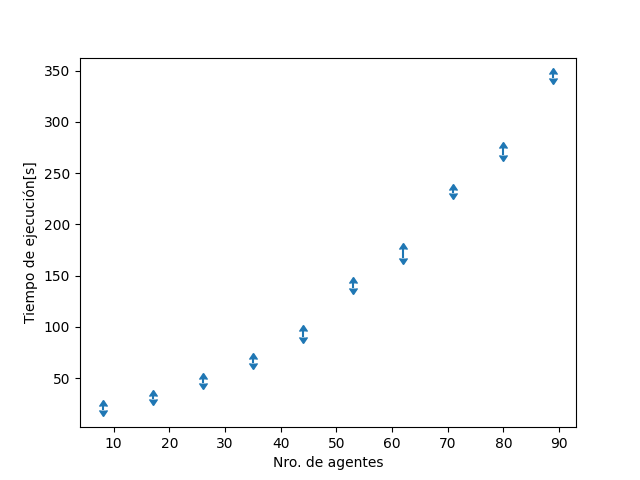
\includegraphics[width=4in]{./images/Antes.png} 
\caption{Tiempos de ejecución antes de las optimizaciones}
\label{fig1}
\end{center}
\end{figure}

\begin{figure}[h]
\begin{center}
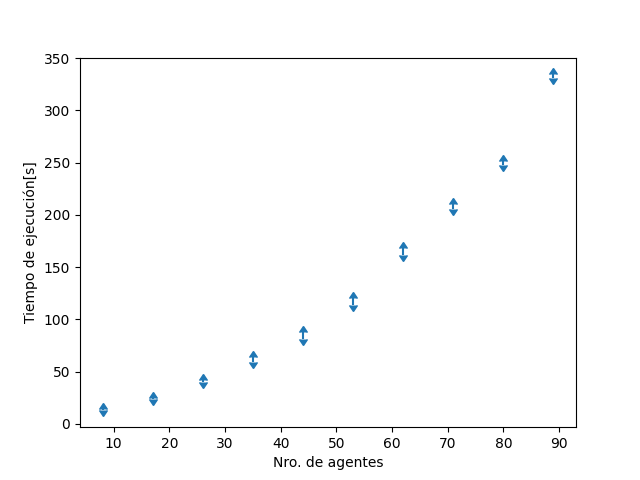
\includegraphics[width=4in]{./images/Despues.png}
\caption{Tiempos de ejecución después de las optimizaciones}
\label{fig2}
\end{center}
\end{figure}

\begin{figure}[h]
\begin{center}
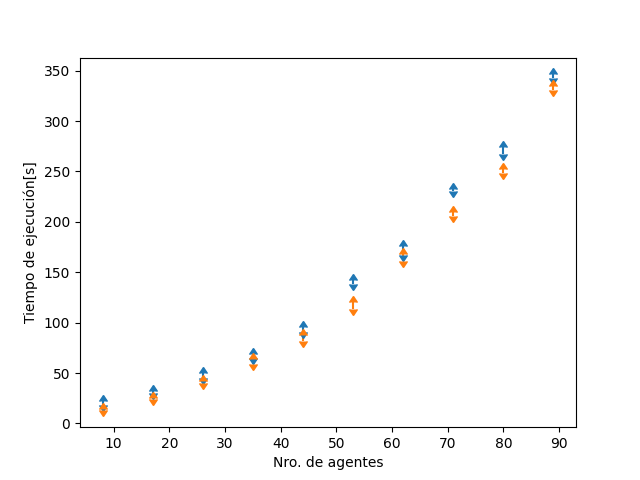
\includegraphics[width=4in]{./images/AntesVSDespues.png}
\caption{Tiempos de ejecución antes de las optimizaciones comparados contra después de las optimizaciones}
\label{fig3}
\end{center}
\end{figure}

\begin{figure}[h]
\begin{center}
\includegraphics[width=4in]{./images/claseCajaImpl.PNG}
\caption{UML implementación de Caja }
\label{cajaImpl}
\end{center}
\end{figure}

\begin{figure}[h]
\begin{center}
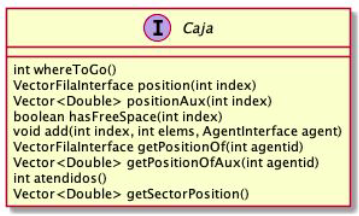
\includegraphics[width=4in]{./images/interfaceCaja.PNG}
\caption{UML interface de Caja }
\label{interfaceCaja}
\end{center}
\end{figure}

\begin{figure}[h]
\begin{center}
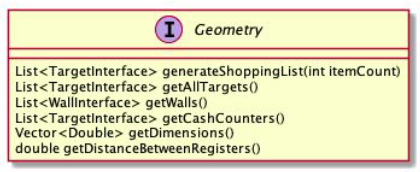
\includegraphics[width=4in]{./images/interfaceGeometry.PNG}
\caption{UML interface de Geometría }
\label{interfaceGeomety}
\end{center}
\end{figure}

\begin{figure}[h]
\begin{center}
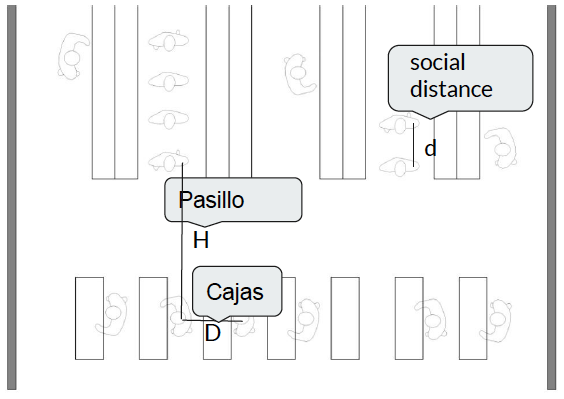
\includegraphics[width=4in]{./images/parametrosSuper.PNG}
\caption{Explicación de parámetros del módulo}
\label{supermercado}
\end{center}
\end{figure}


\clearpage

\section{Tablas}
\begin{table}[h]
\begin{center}
\begin{tabularx}{0.8\textwidth} { 
  | >{\raggedright\arraybackslash}X 
  | >{\centering\arraybackslash}X 
  | >{\raggedleft\arraybackslash}X | }
 \hline
 Estado & Numero \\
 \hline
 Going  & 1 \\
\hline
 Aproximating  & 2 \\
\hline
 Buying & 3  \\
\hline
 Living  & 4  \\
\hline
 Queueing  & 5  \\
\hline
\end{tabularx}
\caption{Representación numérica de los estados en los archivos de salida}
\label{Representación numérica de los estados en los archivos de salida}
\end{center}
\end{table}

\begin{table}[h]
\begin{center}
\begin{tabularx}{0.8\textwidth} { 
  | >{\raggedright\arraybackslash}X 
  | >{\centering\arraybackslash}X 
  | >{\raggedleft\arraybackslash}X | }
 \hline
dt2 & archivos generados \\
 \hline
 0.01 | 0.001 | 0.0001 & 1.txt	2.txt	3.txt	4.txt	5.txt 6.txt	7.txt	8.txt	9.txt \\
\hline
0.1 & 2.txt	3.txt	4.txt	5.txt	6.txt	7.txt	8.txt	9.txt \\
\hline
0.2 & 3.txt	5.txt	6.txt	8.txt  \\
\hline
0.3 & 3.txt	6.txt	9.txt  \\
\hline
0.4  & 5.txt	8.txt  \\
\hline
0.5 & 5.txt \\
\hline
\hline
\end{tabularx}
\caption{Implementación del Tiempo en el Main}
\label{Implementación del Tiempo en el Main}
\end{center}
\end{table}

\begin{table}[h]
\begin{center}
\begin{tabularx}{0.8\textwidth} { 
  | >{\raggedright\arraybackslash}X 
  | >{\centering\arraybackslash}X 
  | >{\raggedleft\arraybackslash}X | }
 \hline
 Parámetro & Valor \\
 \hline
 N  & 8 \\
\hline
 Delta  & 20 \\
\hline
 max & 8  \\
\hline
H & 5  \\
\hline
d  & 2  \\
\hline
p0x  & 0  \\
\hline
p0y  & 0  \\
\hline
\end{tabularx}
\caption{Parámetros del módulo geometria aislado}
\label{Parametros del módulo geometria aislado}
\end{center}
\end{table}

\begin{table}[h]
\begin{center}
\begin{tabularx}{0.8\textwidth} { 
  | >{\raggedright\arraybackslash}X 
  | >{\centering\arraybackslash}X 
  | >{\raggedleft\arraybackslash}X | }
 \hline
Parámetro & Valor \\
 \hline
MOM & CPM \\
\hline
dt  & 0.05 \\
\hline
dt2 & 1  \\
\hline
total & 1200  \\
\hline
\end{tabularx}
\caption{Parámetros del simulador integrado}
\label{Parámetros del simulador integrado}
\end{center}
\end{table}

\begin{table}[h]
\begin{center}
\begin{tabularx}{0.8\textwidth} { 
  | >{\raggedright\arraybackslash}X 
  | >{\centering\arraybackslash}X 
  | >{\raggedleft\arraybackslash}X | }
 \hline
Nro. de Agentes & Promedio & Desviación Estándar \\
 \hline
8 & 20.572 & 2.0435 \\
\hline
17 & 31.1336 & 1.0054 \\
\hline
26 & 47.343 & 2.243 \\
\hline
35 & 66.834 & 1.736 \\
\hline
44 & 93.247 & 2.837 \\
\hline
53 & 140.383 & 2.156 \\
\hline
62 & 171.759 & 4.647 \\
\hline
71 & 231.938 & 1.109 \\
\hline
80& 270.878 & 3.671 \\
\hline
89 & 344.437 & 1.853 \\
\hline

\end{tabularx}
\caption{Tiempos de ejecución antes de las optimizaciones}
\label{Tiempos de ejecución antes de las optimizaciones}
\end{center}
\end{table}

\begin{table}[h]
\begin{center}
\begin{tabularx}{0.8\textwidth} { 
  | >{\raggedright\arraybackslash}X 
  | >{\centering\arraybackslash}X 
  | >{\raggedleft\arraybackslash}X | }
 \hline
Nro. de Agentes & Promedio & Desviación Estándar \\
 \hline
8 & 13.5426 & 0.5934 \\
\hline
17 & 24.6086 & 0.5265 \\
\hline
26 & 41.1566 & 1.2136 \\
\hline
35 & 61.391 & 2.347 \\
\hline
44 & 84.637 & 2.968 \\
\hline
53 & 117.062 & 3.665 \\
\hline
62 & 165.062 & 3.357 \\
\hline
71 & 207.8574 & 2.347 \\
\hline
80& 250.0566 & 2.025 \\
\hline
89 & 332.699 & 1.796 \\
\hline

\end{tabularx}
\caption{Tiempos de ejecución después de las optimizaciones}
\label{Tiempos de ejecución después de las optimizaciones}
\end{center}
\end{table}

\clearpage


\end{document}